\documentclass[xcolor={dvipsnames}]{beamer} % dvipsnames gives more built-in colors
\mode<presentation>

\usetheme{Boadilla}

\definecolor{GWdarkblue}{HTML}{033C5A}

\usecolortheme[named=GWdarkblue]{structure}

% Sets the font
\usepackage[defaultfam,tabular,lining]{montserrat}
% Capital case titles
\setbeamerfont{title}{shape=\scshape}
\setbeamerfont{frametitle}{shape=\scshape}

%Remove "Figure" from captions
\setbeamertemplate{caption}{\raggedright\insertcaption\par}

\usepackage{graphicx}
\usepackage{hyperref}

\title[Introduction]{Introduction to Data Analysis}
\author[SMPA 2152]{Data Analysis for Journalism and Political Communication (Fall 2023)}
\date{Prof. Bell}

\begin{document}

%%%%%%%%%%%%%%%%%%%%%%%%%%%%%%%%%%%%%%%%%%%%%%%%%%%%%%%%%%%%%%%%%%
\frame{
    \titlepage
}

%%%%%%%%%%%%%%%%%%%%%%%%%%%%%%%%%%%%%%%%%%%%%%%%%%%%%%%%%%%%%%%%%%
\frame{
    \frametitle{Chalabi: 3 Ways to Spot a Bad Statistic}
    \centering
    \href{https://www.ted.com/talks/mona_chalabi_3_ways_to_spot_a_bad_statistic}{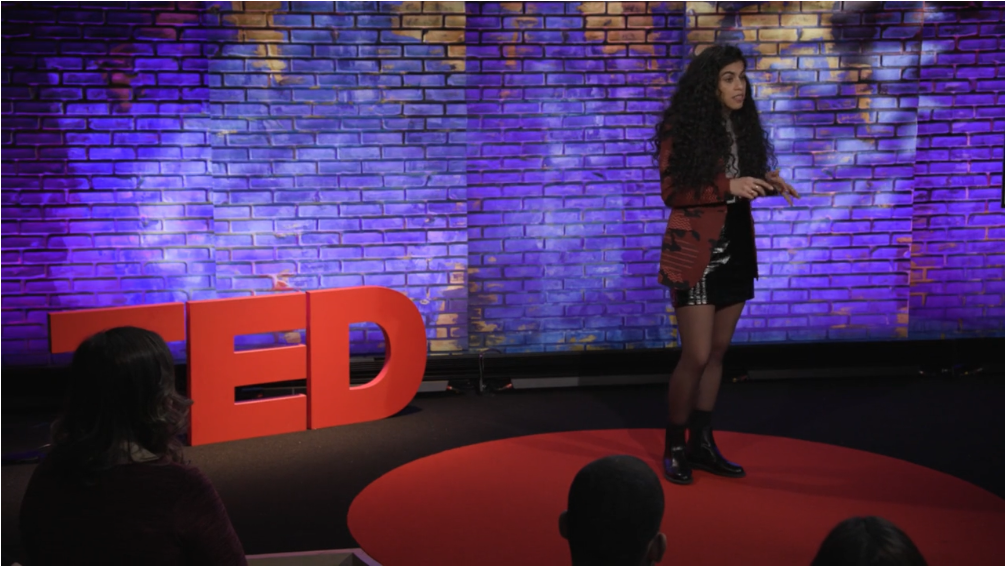
\includegraphics[height = .6\textheight]{chalabi-ted-talk.png}}
    
    \pause
    \begin{enumerate}
        \item Can you see uncertainty?
        \item What is the context of the data (can you see yourself)?
        \item How was the data collected?
    \end{enumerate}
}

%%%%%%%%%%%%%%%%%%%%%%%%%%%%%%%%%%%%%%%%%%%%%%%%%%%%%%%%%%%%%%%%%%
\frame{
    \frametitle{Can you see the uncertainty?}
    \begin{itemize}[<+->]
        \item We rarely get a complete count of everything
        \item Humans do not do well with probability \\
            \only<3>{
                \begin{center}
                    \begin{minipage}{.8\textwidth}
                        \begin{block}{}
                            ``There are only five probabilities the average human can handle: 99 percent, one percent, 100 percent, zero, and 50-50. That's it.'' \\ - Richard Thaler, Nobel Laureate in Economics
                        \end{block}
                    \end{minipage}
                \end{center}
            }
            \only<4>{
                
\includegraphics[height = .25\textwidth]{dc_lottery.png}
            } 
            \only<5>{
                ~\\
                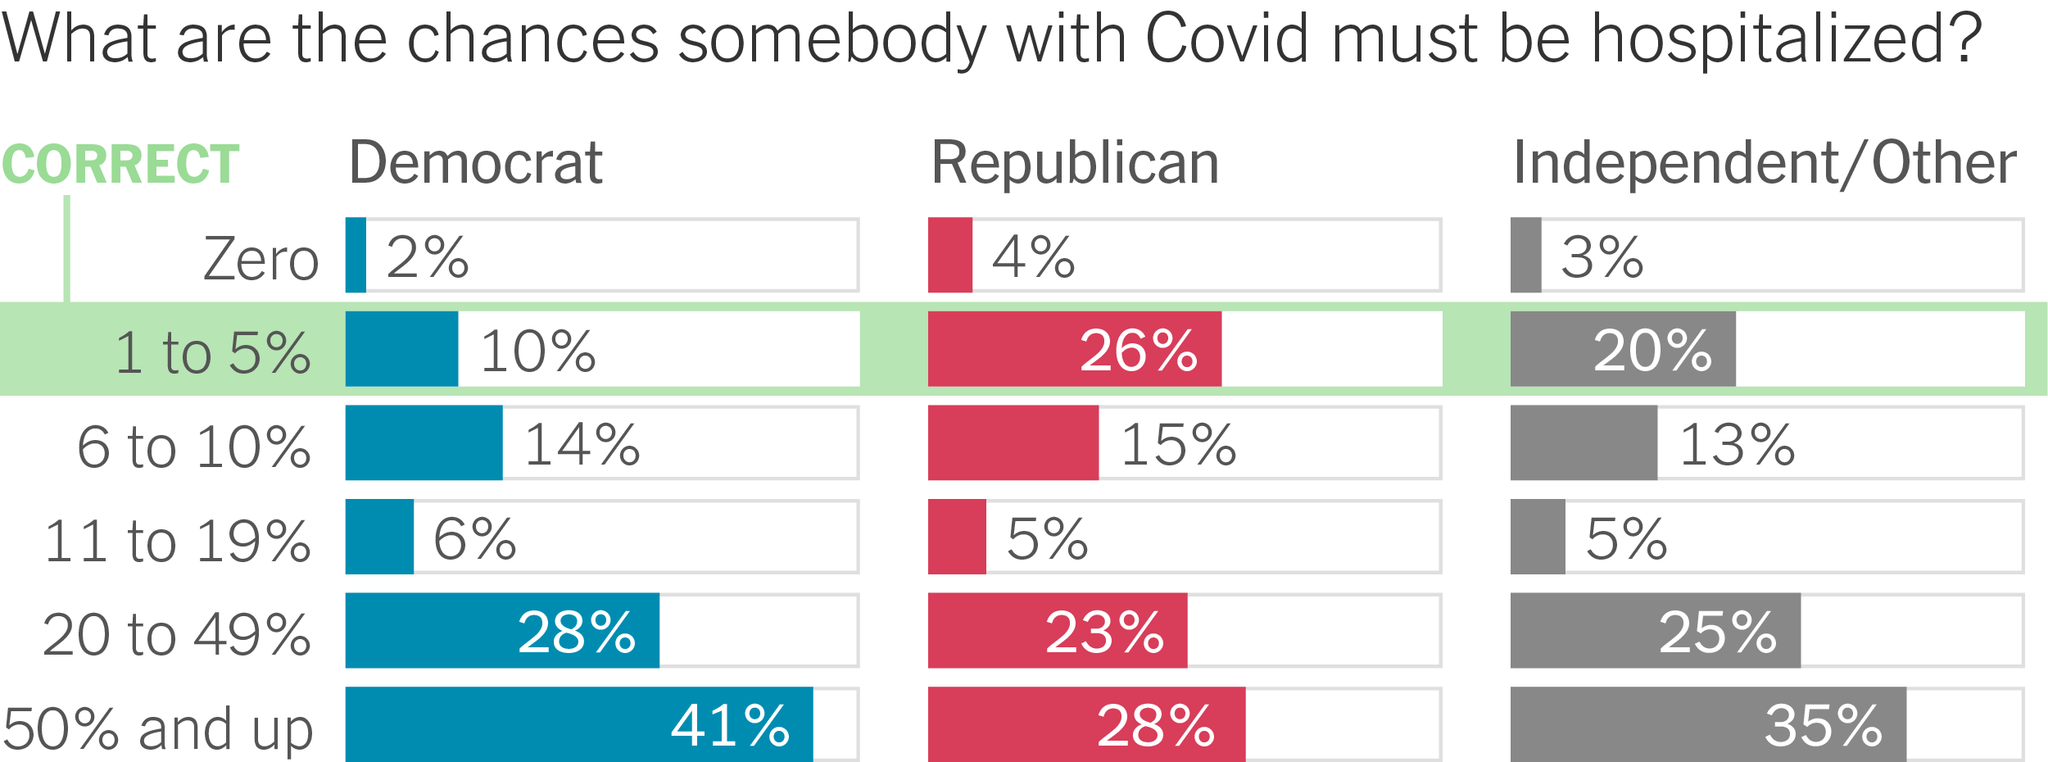
\includegraphics[height = .25\textwidth]{covid_risk.png} \\ \tiny{Source: Franklin Templeton-Gallup Economics of Recovery Study (2020)}
            }
            \only<6->{
                ~\\
                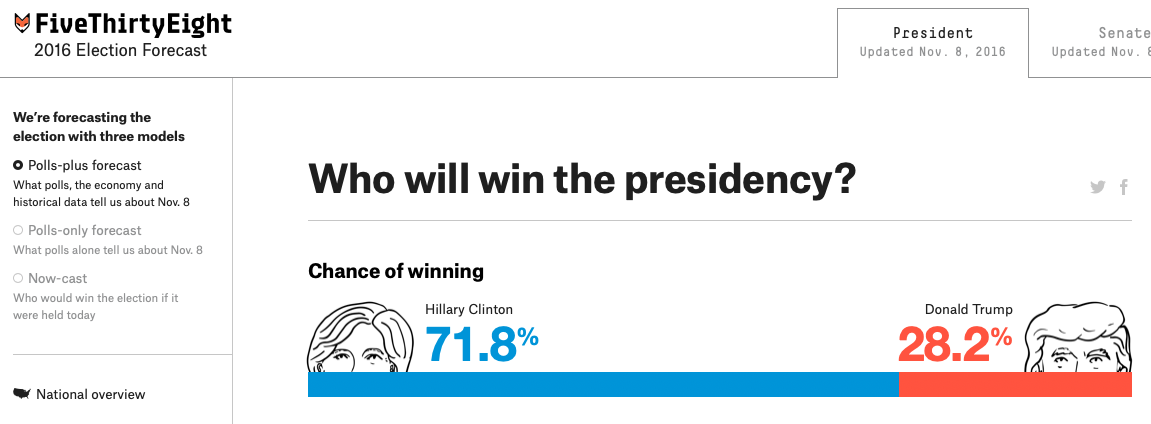
\includegraphics[height = .25\textwidth]{538_2016ElectionForecast.png}
            } 
        \item<7-> We will learn about how to measure and communicate about uncertainty
    \end{itemize}
}

%%%%%%%%%%%%%%%%%%%%%%%%%%%%%%%%%%%%%%%%%%%%%%%%%%%%%%%%%%%%%%%%%%
\frame{
    \frametitle{What is the context of the data?}
    \only<1-4,6->{
        \begin{itemize}[<+->]
            \item<1-4,6-> Some data is produced by unscrupulous actors \\
                \only<1>{~\\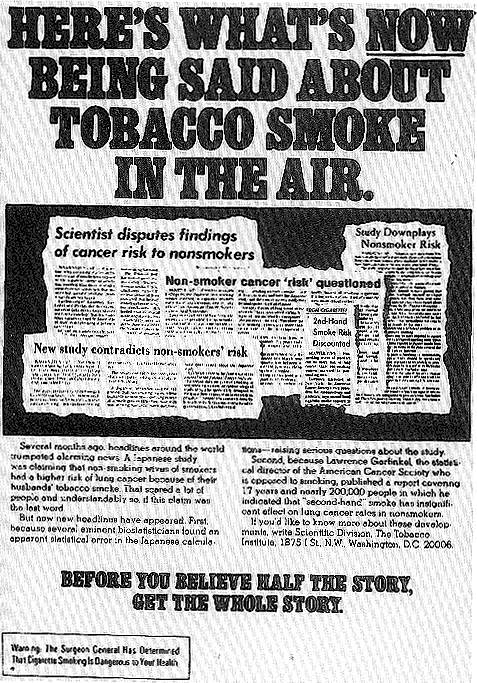
\includegraphics[height = .6\textheight]{tobacco_institute.png}}
                \only<2>{~\\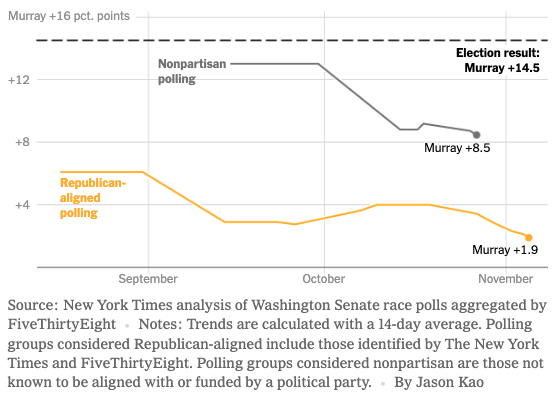
\includegraphics[height = .6\textheight]{patty_murray.png}}
            \item<3-4,6-> But most of the time, poor analysis is not nefarious -- humans are imperfect
            \item<4,6-> We will talk about researcher choices, biases, and assumptions
            \item<6-> We will learn about causation vs. correlation and the importance of theory in making sense of data \\
                \only<7>{~\\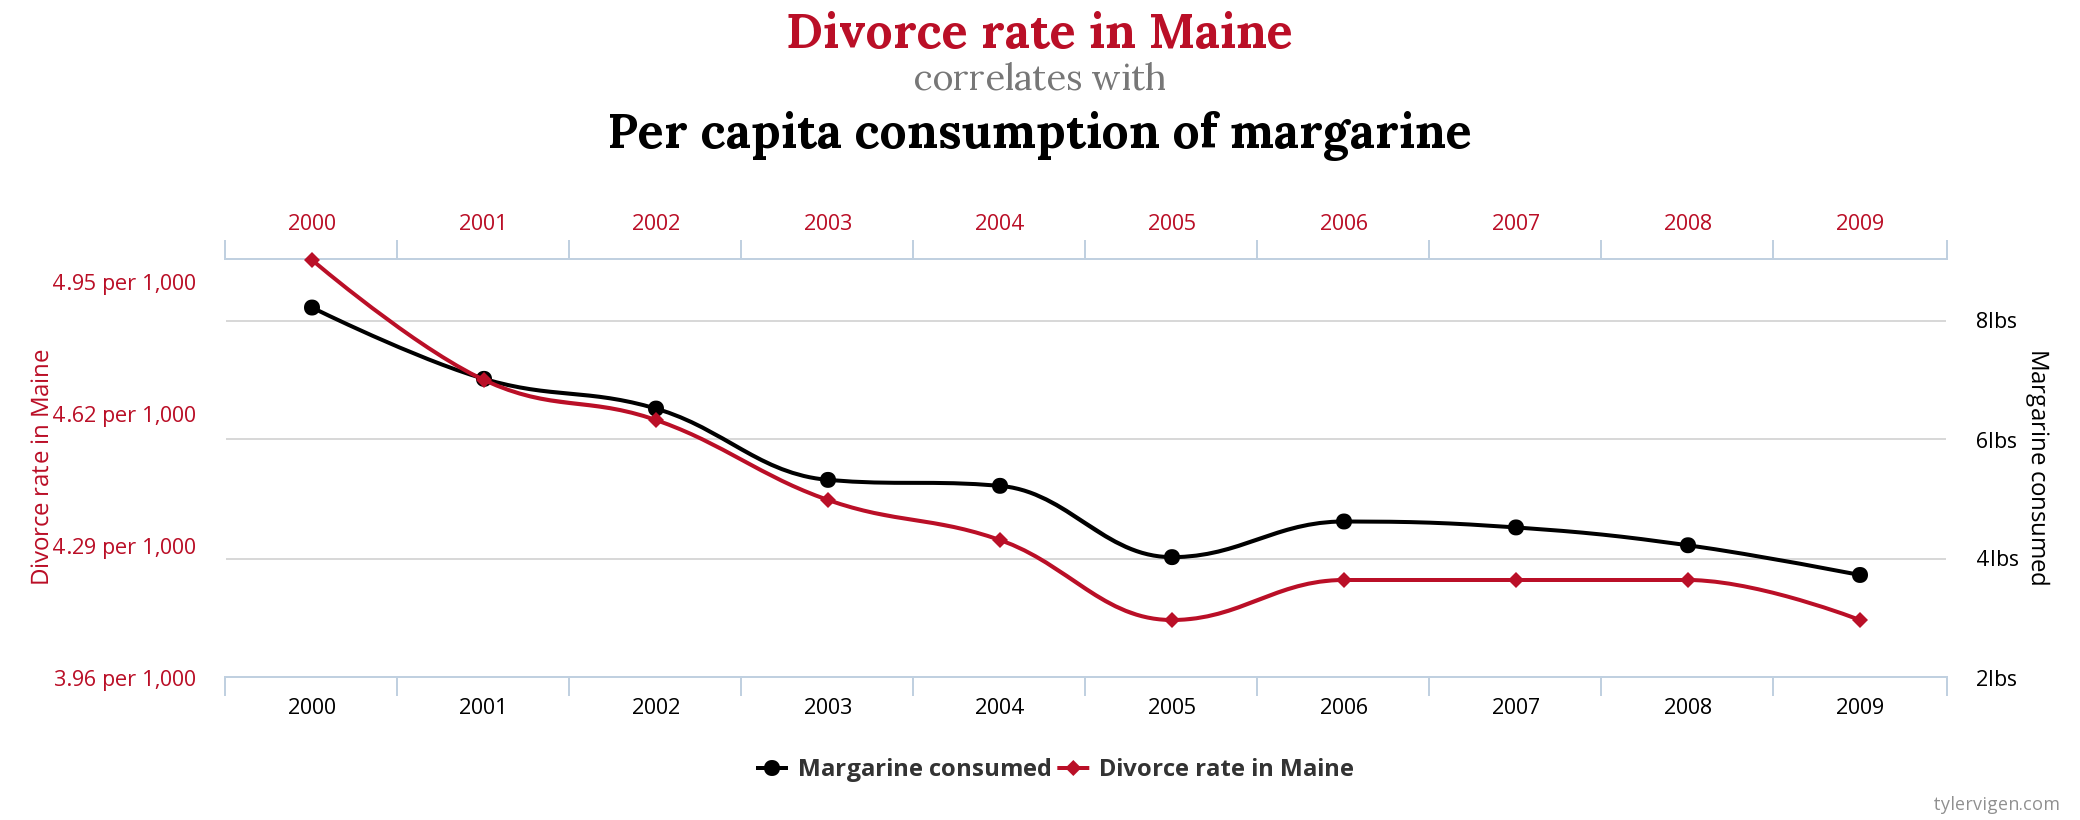
\includegraphics[height = .3\textheight]{spuriouscorrelation.png}}
        \end{itemize}
    }
    \only<5>{
        \centering 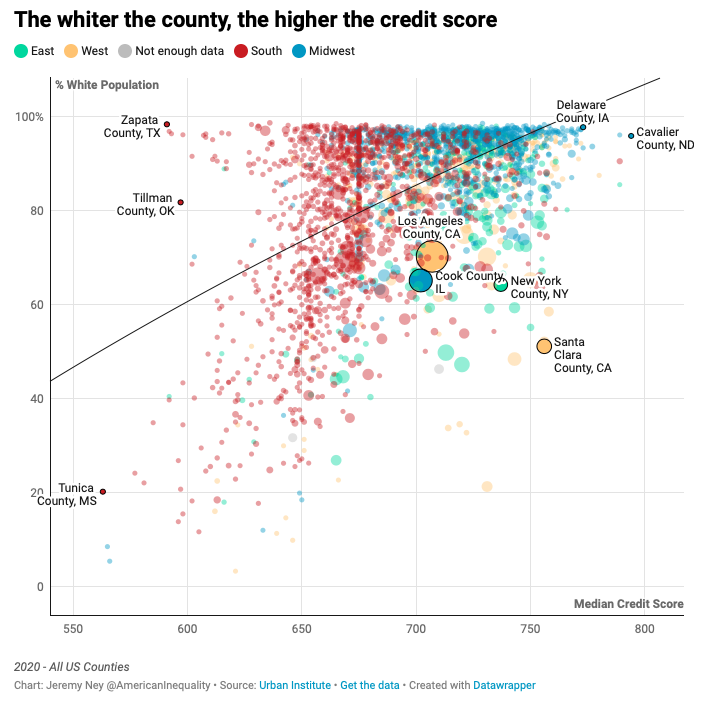
\includegraphics[height = .8\textheight]{CreditScoreInequality.png}
    }
}

%%%%%%%%%%%%%%%%%%%%%%%%%%%%%%%%%%%%%%%%%%%%%%%%%%%%%%%%%%%%%%%%%%
\frame{
    \frametitle{How was the data collected?}
    \only<1-5>{
        \begin{itemize}[<+->]
            \item Data is not objective -- it is generated by humans
            \item Garbage in = garbage out: no amount of statistical wizardry can compensate for bad data
            \item We will spend a lot of time thinking about the \textbf{data generating process} and how it can bias our results \\
                \only<4-5>{~\\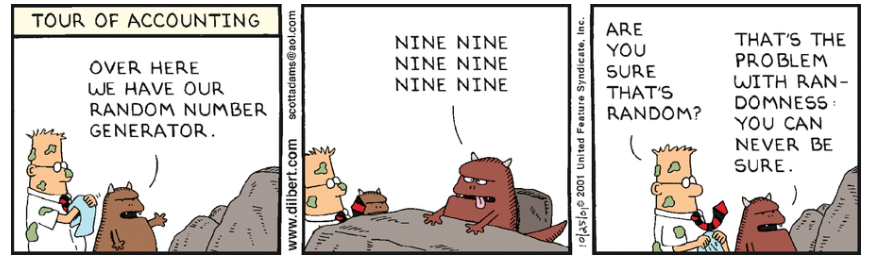
\includegraphics[width = .8\textwidth]{dilbert_randomness.png}}
            \item<5> We will also discuss our ethical responsibilities around data
        \end{itemize}
    }
    \only<6>{
        \centering
        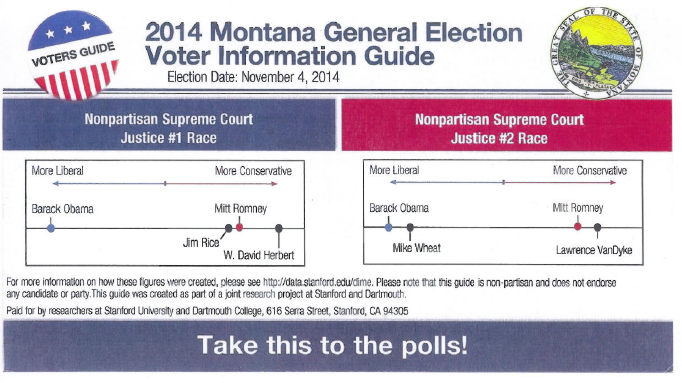
\includegraphics[width = .9\textwidth]{montana_experiment.png}
    }
}

%%%%%%%%%%%%%%%%%%%%%%%%%%%%%%%%%%%%%%%%%%%%%%%%%%%%%%%%%%%%%%%%%%
\frame{
    On your notecard, please write:
    \begin{enumerate}
        \item Preferred name
        \item Preferred pronouns
        \item Year in school and major
        \item Your background in coding and/or statistics
        \item One thing you hope to get out of this class
    \end{enumerate}
}

\end{document}
